\documentclass[10pt]{article}
\usepackage{tikz}
\usetikzlibrary{arrows.meta, positioning}

\usepackage{parskip}
\usepackage[margin=1in]{geometry} 
\usepackage{amsmath,amsthm,amssymb, graphicx, multicol, array}
\usepackage{enumitem}
\usepackage{amssymb}
\usepackage{float}
\usepackage{href-ul}
 
\newcommand{\N}{\mathbb{N}}
\newcommand{\Z}{\mathbb{Z}}
 
\newenvironment{problem}[2][Problem]{\begin{trivlist}
\item[\hskip \labelsep {\bfseries #1}\hskip \labelsep {\bfseries #2.}]}{\end{trivlist}}

\begin{document}
 
\title{State-space model and the Kalman filter}
\author{Jakob Sverre Alexandersen\\
GRA4159 Trends, Cycles \& Signals Extraction\\
Lecture 9}
\maketitle

\tableofcontents
\newpage

\section{Recap}
\begin{itemize}
    \item We now know some of the fundamentals of time series analysis 
    \item We know well the difference between stationary and non-stationary variables and time series processes, such as: 
    \begin{itemize}
        \item AR, MA, RW 
    \end{itemize}
    \item We also know why we sometimes want to focus on trend and cycle decompositions and how to compute them using different methods 
    \item We also now know how to formulate, estimate, and predict the future with a popular type of multivariate time series model 
    \begin{itemize}
        \item VAR 
    \end{itemize}
\end{itemize}
\section{Why state-space and Kalman filter?}
\begin{itemize}
    \item Highly useful tool for nealy all inference promblems in macroeconomics and finance: 
    \begin{itemize}
        \item Can be applied to univariate and multivariate problems 
        \item Can be applied to stationary and non-stationary processes 
        \item Can infer latent states and missing values 
    \end{itemize}
    \item Originally developed to track rockets lol
\end{itemize}
\section{State-space representation}

Observation equation: 
\begin{gather*}
    y_t = H\beta_t + Az_t + e_t
\end{gather*}
Transition equation: 
\begin{gather*}
    \beta_t = \tilde{\mu} + F\beta_{t - 1} + v_t
\end{gather*}
with
\begin{gather*}
    \begin{bmatrix}
        e_t \\
        v_t
    \end{bmatrix}
    \sim \text{i.i.d.} \left(
        \begin{bmatrix}
            0 \\ 0
        \end{bmatrix},
        \begin{bmatrix}
            R & 0 \\
            0 & Q
        \end{bmatrix}
    \right)
\end{gather*}
Definitions: 
\begin{itemize}
    \item $y_t $: $(n\times 1) $ vector of observable variables 
    \item $\beta_t $: ($k\times 1) $ vector of (unobserved) state variables 
    \item $z_t $: $(r \times 1) $ vector of exogenous observed variables 
    \item $e_t, v_t $: $(n\times 1) \text{ and }(k\times 1) $ vectors of measurement and transition equation errors 
    \item $H, A, F, \tilde{\mu} $: $(n\times k), (n\times r), (k\times k), \text{ and }(k\times 1)$ parameter matrices 
    \item $R, Q $: $(n\times n)\text{ and }(k\times k) $ covariance matrices 
\end{itemize}

The observation equation is just $n $ linear equations 
\begin{itemize}
    \item Often, but not always, $R $ is assumed to be diagonal, i.e., $n $ independent linear static equations 
\end{itemize}
The transition equation follows a VAR structure. Note: $R \text{ and } Q $ are assumed to be independent (can be relaxed, but not now).
\newpage 
\subsection{VAR models in state-space form }
\begin{itemize}
    \item Nearly all linear models can be written in state-space form (VAR, ARMA, UC etc.)
    \item Consider the VAR model:
    \begin{gather*}
        \begin{bmatrix}
            y_{1, t}\\
            y_{2, t}
        \end{bmatrix}
        = \begin{bmatrix}
            1 \\ 1
        \end{bmatrix}
        + \begin{bmatrix}
            0.5 & 0 \\
            1 & 0.2
        \end{bmatrix}
        \begin{bmatrix}
            y_{1, t - 1}\\
            y_{2, t - 1}
        \end{bmatrix}
        + \begin{bmatrix}
            v_{1, t}\\
            v_{2, t}\\
        \end{bmatrix}
    \end{gather*}
    with 
    \begin{gather*}
        \begin{bmatrix}
            v_{1, t}\\
            v_{2, t}\\
        \end{bmatrix}
        \sim \text{i.i.d.} N\left(
            \begin{bmatrix}
                0 \\ 0
            \end{bmatrix},
            \begin{bmatrix}
                1 & 0.2 \\
                0.2 & 1
            \end{bmatrix}
        \right)
    \end{gather*}
    Written in a state-space representation we get the measurement equation: 
    \begin{gather}
        \begin{bmatrix}
            v_{1, t}\\
            v_{2, t}\\
        \end{bmatrix}
        = 
        \begin{bmatrix}
            1 & 0 \\
            0 & 1
        \end{bmatrix}
        \begin{bmatrix}
            \beta_{1, t}\\
            \beta_{2, t}\\
        \end{bmatrix}
    \end{gather}
    and the associated transition equation: 
    \begin{gather*}
        \begin{bmatrix}
            \beta_{1, t}\\
            \beta_{2, t}\\
        \end{bmatrix}
        = 
        \begin{bmatrix}
            1\\
            1\\
        \end{bmatrix}
        + 
        \begin{bmatrix}
            0.5 & 0\\
            1 & 0.2
        \end{bmatrix}
        \begin{bmatrix}
            \beta_{1, t - 1}\\
            \beta_{2, t -1 }\\
        \end{bmatrix}
        + \begin{bmatrix}
            v_{1, t}\\
            v_{2, t}
        \end{bmatrix}
    \end{gather*}
    Accordingly, $n = 2,\, k = 2,\, r = 0 $ and: 
    \begin{gather*}
        H = \begin{bmatrix}
            1 & 0 \\
            0 & 1
        \end{bmatrix}
        \quad \tilde{\mu} = \begin{bmatrix}
            1 \\ 1
        \end{bmatrix}
        \quad F = \begin{bmatrix}
            0.5 & 0 \\
            1 & 2
        \end{bmatrix}
        \quad Q = \begin{bmatrix}
            1 & 0.2 \\
            0.2 & 1
        \end{bmatrix}
    \end{gather*}
    $z_t = 0 \text{ and } e_t = 0\,\forall t $, i.e., no exogenous variables and no measurement errors
    \item But, in state-space form, more than one way of rewriting a model 
    \item In the case just described we could for example have set $r = 1 $, and let $\tilde{\mu} = \begin{bmatrix} 0 & 0 \end{bmatrix}' $, yielding the state-space representation: 
    \begin{gather}
        \begin{bmatrix}
            y_{1, t}\\
            y_{2, t}\\
        \end{bmatrix}
        = \begin{bmatrix}
            1 & 0 \\
            0 & 1
        \end{bmatrix}
        \begin{bmatrix}
            \beta_{1, t}\\
            \beta_{2, t }\\
        \end{bmatrix}
        +
        \begin{bmatrix}
            1\\
            1\\
        \end{bmatrix}\\
        \begin{bmatrix}
            \beta_{1, t}\\
            \beta_{2, t }\\
        \end{bmatrix}
        = 
        \begin{bmatrix}
            0.5 & 0 \\ 
            1 & 0.2
        \end{bmatrix}
        \begin{bmatrix}
            \beta_{1, t - 1}\\
            \beta_{2, t -1 }\\
        \end{bmatrix}
        +
        \begin{bmatrix}
            v_{1, t}\\
            v_{2, t}\\
        \end{bmatrix}\notag
    \end{gather}
    In (1) $\beta_{i, t} = y_{i, t}, \text{ while in (2) }\beta_{i, t} = y_{i, t} - \tilde{\mu}_i = y_{i, t} - 1 \text{ for }i = 1,\, 2 $
\end{itemize}
\newpage 
\subsection{ARMA models in state-space form}
Consider the ARMA(1, 1) model: 
\begin{gather*}
    y_t = \phi_1y_{t - 1} + \epsilon_t + \theta\epsilon_{t -1 }\Rightarrow (1 - \theta L)y_t = (1 + \theta L)\epsilon_t
\end{gather*}
Put in state-space form 
\begin{gather*}
    y_t = \begin{bmatrix}
        1 & \theta 
    \end{bmatrix}
    \begin{bmatrix}
        \beta_{1, t}\\
        \beta_{2, t}\\
    \end{bmatrix}
    \text{ and }
    \begin{bmatrix}
        \beta_{1, t}\\
        \beta_{2, t}\\
    \end{bmatrix}
    = 
    \begin{bmatrix}
        \phi & 0 \\ 
        1 & 0
    \end{bmatrix}
    \begin{bmatrix}
        \beta_{1, t - 1}\\
        \beta_{2, t -1 }\\
    \end{bmatrix}
    + \begin{bmatrix}
        \epsilon_t \\ 
        0
    \end{bmatrix}
\end{gather*}
with first line from transition question and observation equation 
\begin{gather*}
    (1 - \phi L)\beta_{1, t} = \epsilon_t \text{ and } y_t = (1 + \theta L)\beta_{1, t}
\end{gather*}
since $\beta_{2, t} = \beta_{1, t - 1} $. Thus 
\begin{gather*}
    y_t = (1 + \theta L)(1 - \phi L)^{-1}\epsilon_t \Rightarrow (1 - \phi L)y_t = (1 + \theta L)\epsilon_t
\end{gather*}
\subsection{Trends and cycle methods recap}
\begin{itemize}
    \item In earlier lectures we talked about different methods for directly estimating the trend and cycle from non-stationary data 
    \item A class of models that are often used for this is called Unobserved Components (UC) models 
    \item As the name suggests, these models contain unobserved components 
    \item The state-space formulation and the Kalman Filter are often used for estimation 
\end{itemize}
\subsection{Unobserved components models}
Consider the following simple model 
\begin{gather*}
    y_t = g_t + c_t 
\end{gather*}
where $g_t $ is the trend and $c_t $ is the cycle 

Assume also that the stochastic trend is driven by a random walk with drift: 
\begin{gather*}
    g_t = \tilde{\mu}_1 + g_{t - 1} + \epsilon_{1, t}
\end{gather*}
and the cyclical component follows a stationary AR(2) model: 
\begin{gather*}
    c_t = \phi_1c_{t - 1} + \phi_2c_{t - 2} + \epsilon_{2, t}
\end{gather*}
where 
\begin{gather}
    \begin{bmatrix}
        \epsilon_{1, t}\\
        \epsilon_{2, t}
    \end{bmatrix}
    \sim \text{i.i.d.} N \left(
        \begin{bmatrix}
            0 \\ 0
        \end{bmatrix},
        \begin{bmatrix}
            \sigma^2_1 & 0 \\ 
            0 & \sigma^2_2
        \end{bmatrix}
    \right)
\end{gather}
\newpage 
Employing the state-space representation we get the following measurement and transition equations:
\begin{gather*}
    y_t = 
    \begin{bmatrix}
        1 & 1 & 0
    \end{bmatrix}
    \begin{bmatrix}
        \beta_{1, t}\\
        \beta_{2, t}\\
        \beta_{2, t - 1}\\
    \end{bmatrix}
\end{gather*}
so that, $\beta_{1, t} = g_t \text{ and }\beta_{2, t} = c_t $
\begin{gather*}
    \begin{bmatrix}
        \beta_{1, t}\\
        \beta_{2, t}\\
        \beta_{2, t - 1}\\
    \end{bmatrix} = 
    \begin{bmatrix}
        \tilde{\mu}\\
        0 \\
        0 \\
    \end{bmatrix}
    + 
    \begin{bmatrix}
        1 & 0 & 0 \\ 
        0 & \phi_1 & \phi_2 \\ 
        0 & 1 & 0
    \end{bmatrix}
    \begin{bmatrix}
        \beta_{1, t - 1}\\
        \beta_{2, t -1}\\
        \beta_{2, t - 2}\\
    \end{bmatrix}
    + 
    \begin{bmatrix}
        \epsilon_{1, t}\\
        \epsilon_{2, t}\\
        0
    \end{bmatrix}
\end{gather*}
Here, $n = 1,\, k = 3,\, r = 0 $, and: 
\begin{gather*}
    H = \begin{bmatrix}
        1 & 1 & 0
    \end{bmatrix}
    \quad \tilde{\mu} \begin{bmatrix}
        \tilde{\mu}_1 \\ 0
    \end{bmatrix}
    \quad F = \begin{bmatrix}
        1 & 0 & 0 \\ 
        0 & \phi_1 & \phi_2 \\ 
        0 & 1 & 0
    \end{bmatrix}
    \quad A = 0
\end{gather*}
and $e_t = 0\, \forall t $. $Q^* $ is given by the covariance matrix in (3), implying that: 
\begin{gather*}
    G = \begin{bmatrix}
        1 & 0 \\
        0 & 1 \\
        0 & 0 \\
    \end{bmatrix}
    \quad Q = 
    \begin{bmatrix}
        \sigma^2_1 & 0 & 0 \\
        0 & \sigma^2_2 & 0 \\ 
        0 & 0 & 0 
    \end{bmatrix}
\end{gather*}
\subsection{State-space form: don't forger}
\begin{itemize}
    \item The state variables do not have to be unobserved in the state-space representation
    \item There are usually many ways of writing a model into state-space form 
    \item Why do we do it?
    \begin{itemize}
        \item Facilitates employing the Kalman Filter 
        \item Facilitates MLE 
        \item Facilitates (conditional) forecasting and inferring missing values 
    \end{itemize}
    \item BUT: subtle issue regarding for identification (not finna look at it :skull:)
\end{itemize}
\newpage 
\section{The Kalman filter}
\begin{itemize}
    \item Once a model is put into state-space form we can utilize the Kalman filter machinery 
    \item The Kalman filter is: 
    \begin{itemize}
        \item A linear filter 
        \item A recursive procedure for computing the optimal estimate of the unobserved state vector 
        \item Provides the minimum squared error estimate of the unobserved state irrespective of the assumptions on the error terms ($R \text{ and } Q $) -- if Gaussian, the filter provides the exact conditional probability 
    \end{itemize} 
    \item The Kalman filter can also be used for MLE 
    \item Consists of two (three) steps: preduction and updating done recursively through time. Once at the end of a sample (step three) smoothing can be applied 
\end{itemize}
\subsection{Some useful definitions}
\begin{itemize}
    \item $\beta_{t|t - 1}$: expectation of $\beta_t $ conditional on information up to $t - 1 $, i.e., $\mathbb{E}[\beta_t|I_{t - 1}] $
    \item $P_{t | t - 1}$: covariance matrix of $\beta_t $ conditional on information up to $t  -1 $, i.e., $\mathbb{E}\left[(\beta_t - \beta_{t|t - 1})(\beta_t - \beta_{t|t - 1})'\right] $
    \item $\beta_{t|t} $: expectation of $\beta_t $ conditional on information up to $t $
    \item $P_{t|t} $: covariance matrix of $\beta_t $ conditional on information up to $t $, i.e., $\mathbb{E}\left[(\beta_t - \beta_{t|t})(\beta_t - \beta_{t|t })'\right] $
    \item $y_{t|t - 1} $: forecast of $y_t $ given information up to time $t - 1 $
    \item $\eta_{t|t - 1} $: forecast error of $y_t $, i.e., $y_t - y_{t|t - 1} $
    \item $f_{t|t - 1} $: conditional covariance of the forecast error, $\eta_{t|t - 1} $, i.e., $\mathbb{E}\left[(y_t - y_{t|t - 1})^2\right] = \mathbb{E}\left[\eta_{t|t - 1}^2\right]$
    \item $\beta_{t|T} $: expectation of $\beta_t $ conditional on information up to $T $, i.e., the whole sample 
    \item $P_{t|T} $: covariance matrix of $\beta_t $ conditional on information up to $T $, i.e., the whole sample $\mathbb{E}\left[(\beta_t -\beta_{t|T})(\beta_t - \beta_{t|T})'\right] $
\end{itemize}
\subsection{Assumptions for now}
\begin{itemize}
    \item $\beta_{0|0}\text{ and }P_{0|0} $ are known (i.e., the initial state and its covariance)
    \item We will also, for now, assume that the parameter matrices, $H,\, A,\, \tilde{\mu},\, F,\, R \text{ and } Q $ are known, and that $z_t $ is known for all $t $
\end{itemize}
\newpage 
\subsection{Prediction, updating, Smoothing}
\subsubsection{Prediction}
At the beginning of time $t $ we want to form an optimal predictor of $y_t $ based on all the available information up to time $t -  1 $, i.e., we want to calculate $y_{t|t - 1} $. We start by predicting the state: 
\begin{gather*}
    \beta_{t|t - 1} = \tilde{\mu} + F\beta_{t- 1|t - 1}
\end{gather*}
with conditional covariance:
\begin{gather*}
    P_{t|t - 1} = FP_{t - 1|t - 1}F' + Q
\end{gather*}
Accordingly, the condition forecast of $y_t $ is:
\begin{gather*}
    y_{t|t - 1} = H\beta_{t|t - 1} + Az_t 
\end{gather*}
\subsubsection{Updating}
Once $y_t $ is realized at the end of time $t $ we can calculate the forecast error, $\eta_{t|t - 1} $ and its associated conditional covariance $f_{t|t - 1} $: 
\begin{gather*}
    \eta_{t|t - 1} = y_t - (H\beta_{t|t - 1} + Az_t) \\
    f_{t|t - 1} = HP_{t|t - 1}H' + R
\end{gather*}
The forecast errors ($\eta_{t|t - 1} $) contain new information about the unobserved state $\beta_t $ beyond that contained in $\beta_{t|t - 1} $. Thus, we can use the new information contained in the forecast errors to update our belief about $\beta_t $, which is the goal of the Kalman Filter recursions.

The updating equations for $\beta_{t|t}\text{ and }P_{t|t} $ follow from employing the multivariate conditional normal distribution, and are: 
\begin{gather*}
    \beta_{t|t} = \beta_{t|t - 1} + K_t\eta_{t|t - 1}\\
    P_{t|t} = P_{t|t - 1} - K_tHP_{t|t - 1}
\end{gather*}
where 
\begin{gather}
    K_t = P_{t|t - 1}H'f_{t|t - 1}^{-1}
\end{gather}
is called the Kalman gain
\newpage 
\subsubsection{Updating and intuition}
\begin{itemize}
    \item $\beta_{t|t} $ is formed as a kind of weighted average of $\beta_{t|t - 1} $ and the new information contained in the forecast error. The weight put on the forecast error is determined by $K_t $, the Kalman gain 
    \item Writing out (4) using the expression for $f_{t|t - 1} $, and for simplicity, assuming that $\beta_{t|t} $ and $H $ have dimensions $(1\times 1)$, we get: 
    \begin{gather*}
        K_t = \frac{1}{H}\frac{P_{t|t - 1}H^2}{P_{t|t - 1}H^2 + R}
    \end{gather*}
    an inverse function of $R $, the covariance of $e_t $, and a positive function of the uncertainty regarding $\beta_{t|t - 1},\text{ i.e., }P_{t|t - 1}$
\end{itemize}
\subsubsection{Preduction and updating summary}
\begin{enumerate}
    \item Set $t = 1 $
    \item Prediction step: 
    \begin{gather*}
        \beta_{t|t - 1} = \tilde{\mu} + G\beta_{t - 1|t - 1}\\
        P_{t|t - 1} = FP_{t -1 |t - 1}F' + Q 
    \end{gather*}
    \item Updating step 
    \begin{gather*}
        \eta_{t|t - 1} = y_t - H\beta_{t|t - 1}-Az_t \\
        f_{t|t - 1} = HP_{t |t - 1}H' + R\\
        \beta_{t|t} = \beta_{t|t - 1} + K_t\eta_{t|t - 1}\\
        P_{t|t} = P_{t|t - 1} - K_tHP_{t|t - 1}
    \end{gather*}
    where 
    \begin{gather*}
        K_t = P_{t|t - 1}H'f_{t|t-1}^{-1}
    \end{gather*}
    \item set $t = t + 1 $, return to 2
\end{enumerate}
\subsubsection{Smoothing}
\begin{itemize}
    \item Notice, the recursive filtering algorithm only uses information up to time $t $ on every recursion 
    \item Smoothing is an interation that runs backward in time, starting from time $t = T $ and going back to time $t = 1 $
    \item A smoothed estimate, denoted $\beta_{t|T} $, might provide us with a more accurate estimate of the unobserved state, simple becuase it uses more information than the basic filter, which gives us $\beta_{t|t} $
    \item Once the basic Kalman filter recursions have been run, we can simply iterate the two following equations backwards for $t = T,\, T - 1, \, \dots, 1 $ to get $\beta_{t|T} $:
    \begin{gather*}
        \beta_{t|T} = \beta_{t|t} + P_{t|t }F'P_{t + 1|t}^{-1}(\beta_{t + 1|T} - F\beta_{t|t}- \tilde{\mu})\\
        P_{t|T} = P_{t|t} + P_{t|t}F'P_{t+1|t}^{-1}(P_{t+1|T} - P_{t + 1|t})P_{t + 1|t}^{-1\prime}FP_{t|t}'
    \end{gather*}
\end{itemize}
\newpage 
\subsection{Missing values, forecasting and starting values}
\begin{itemize}
    \item If the observable vector $y_t $ contains missing values for some or more of the $n $ variables, the Kalman filter machinery can still be used 
    \item When all observations are missing -- the updating step will not be conducted 
    \item If only some observations are missing, updating will be done, but only conditional on the information in the observed observations 
    \item Thus, the Kalman filter can easily be used for inferring missing values in the observables, and for conditional forecasting
    \item To run the Kalman filter recursions for $t = 1, 2, \dots, T $, we need some starting values -- we need $\beta_{0|0}\text{ and }P_{0|0}$
    \item In choosing $\beta_{0|0}\text{ and }P_{0|0}$ we will separate between two cases: 
    \begin{itemize}
        \item For stationary state variable processes, the unconditional mean and covariance matrix of $\beta_t $ may be employed as $\beta_{0|0}\text{ and }P_{0|0}$, respectively. That is: $\beta_{0|0} = (I_k - F)^{-1}\tilde{\mu}\text{ and } \text{vec}(P_{0|0}) = (I_k - F \otimes F)^{-1}\text{vec}(Q) $
        \item Second, for nonstationary state variable processes, the unconditional mean and covariance matrix of $\beta_t $ do not exist. Accordingly, $\beta_{0|0} $ can be set at any arbitrary $(k\times 1) $ vector (i.e., wild guessing). To assign a very large uncertainty to this guess, we should assign very large values to the diagonal elements of $P_{0|0} $.
    \end{itemize}
\end{itemize}
\section{Filtering examples}
\begin{figure}[H]
    \centering
    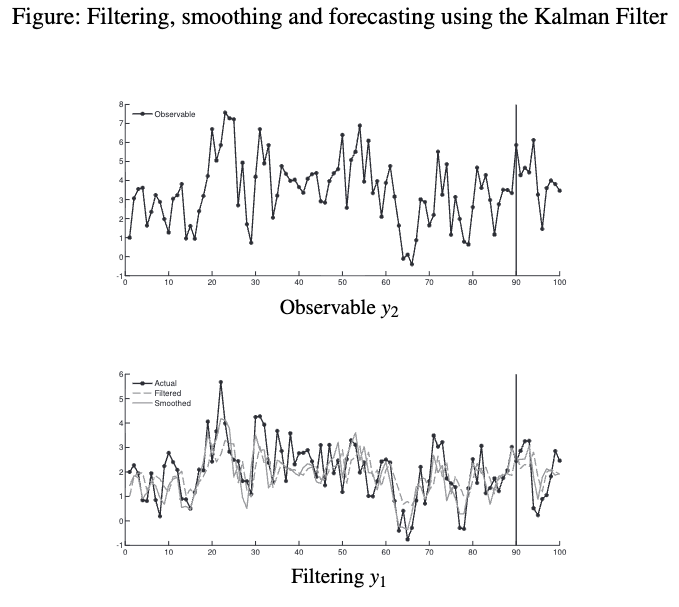
\includegraphics[width=0.6\textwidth]{2026-03-11-15-58-03.png}
\end{figure}
\newpage 
\begin{figure}[H]
    \centering
    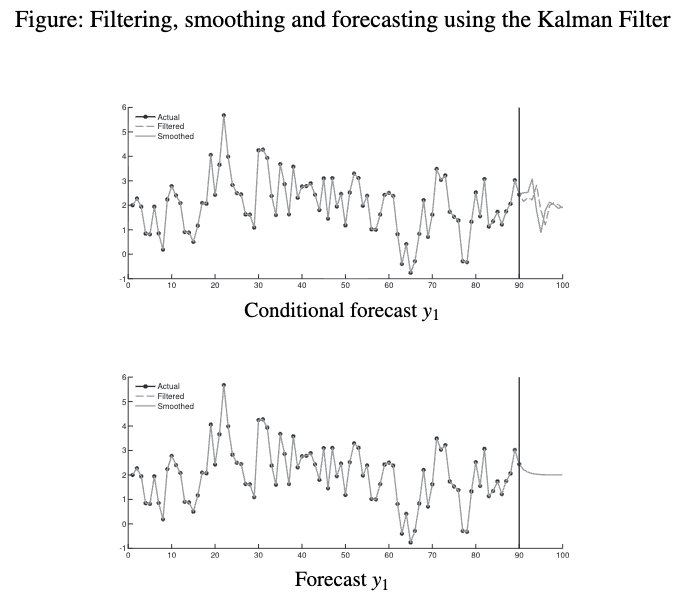
\includegraphics[width=0.6\textwidth]{2026-03-11-15-58-45.png}
\end{figure}
\section{Kalman filter and MLE}
\begin{itemize}
    \item Up until now assumed that $H,\, A,\, \tilde{\mu},\, F,\, R \text{ and } Q $ are known 
    \item The Kalman filter can also be used to get the maximum likelihood estimate of these parameters 
    \item To do so we utilize the prediction error decomposition of the log likelihood function:
    \begin{gather}
        \ln L(\theta|\tilde{y}_T) = \sum_{t = 1}^{T}\left[- \frac{1}{2}\ln\big((2\pi)^n|f_t|\big) - \frac{1}{2}\sum_{t = 1}^{T}\left(\eta_{t}'f_t^{-1}\eta_t\right)\right]
    \end{gather}
    \item (5) is a function of $\eta_t \text{ and } f_t $ -- derived within the KF iterations 
    \item Thus, at each iteration of the filter, we can compute: 
    \begin{gather*}
        l(\theta) = l(\theta) - \frac{1}{2}\ln\big((2\pi)^n|f_{t - 1}|\big) - \frac{1}{2}\left(\eta_{t|t - 1}'f_{t|t - 1}^{-1}\eta_{t|t - 1}\right)
    \end{gather*}
\end{itemize}
\newpage 
\section{The Kalman filter and MLE example}
\begin{figure}[H]
    \centering
    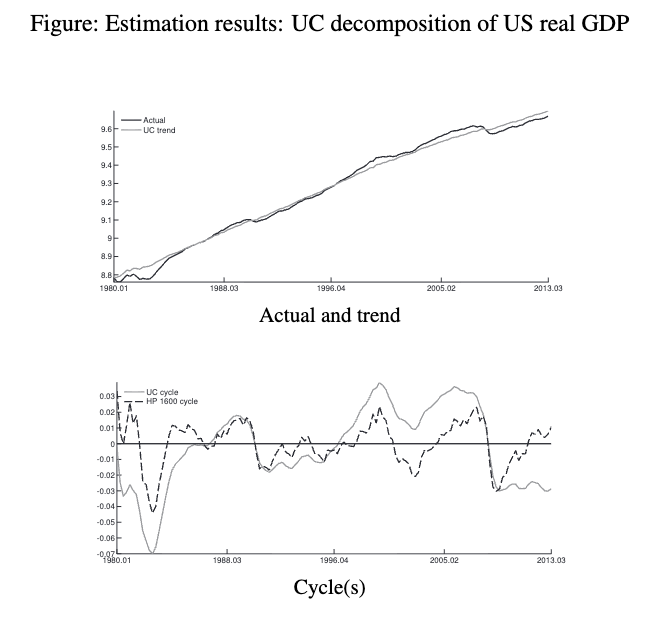
\includegraphics[width=0.8\textwidth]{2026-03-11-16-04-11.png}
\end{figure}
\section{Summary}
\begin{enumerate}
    \item The state-space representation consists of an observation equation and a transition equation. Nearly all linear models in economics can be put into a state-space representation
    \item The Kalman filter is a recursive filter that can be used for estimating unobserved state variables, infer missing values among the observed variables, forecasting, and parameter estimation. 
    \item The Kalman filter consists of two steps: a prediction step followed by an updating step. Sometimes a third step is also added to the procedure, namely a smoothing step 
    \item When the parameters of the model are unknown, the Kalman filter together with the state-space representation can be used for MLE 
\end{enumerate}
\end{document}